% Minimal TikZ standalone example
\documentclass[tikz, border=1mm]{standalone}

\usepackage{amsmath}
\usepackage{tikz}

\usetikzlibrary{calc,angles,quotes}

\begin{document}

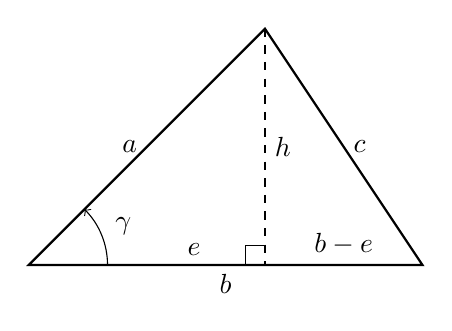
\begin{tikzpicture}[scale=1.0]
	% Points
	\coordinate (A) at (0,0);
	\coordinate (C) at (5,0);
	\coordinate (B) at (3,3);

	% Feet of altitude from B to AC
	\coordinate (D) at (3,0);

	% Triangle sides
	\draw[thick] (A) -- (B) -- (C) -- cycle;

	% Altitude
	\draw[dashed] (B) -- (D);

	% Right angle marker
	\pic [draw, angle radius=7pt, angle eccentricity=1]
	{right angle = B--D--A};

	% Side labels
	\node[left]  at ($(A)!0.5!(B)$) {$a$};
	\node[below] at ($(A)!0.5!(C)$) {$b$};
	\node[right] at ($(B)!0.5!(C)$) {$c$};

	% Angle gamma
	\pic[draw, ->, "$\gamma$", angle eccentricity=1.3, angle radius=1cm]
	{angle = C--A--B};

	% Segment labels on altitude projection
	\node[above] at ($(A)!0.7!(D)$) {$e$};
	\node[above] at ($(D)!0.5!(C)$) {$b-e$};

	% Height label
	\node[right] at ($(B)!0.5!(D)$) {$h$};
\end{tikzpicture}

\end{document}
